\chapter{Preliminaries}

\begin{figure}
	\centering
	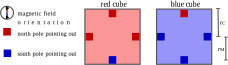
\includegraphics[width=0.70\textwidth]{figures/magnetic_cubes.pdf}
	\caption{Simplified top-down view of the two magnetic modular cube types with their outwards pointing magnet poles, illustrated as red and blue squares. Also visualizes the lengths $r_C$ and $r_M$}
	\label{fig:magnetic_cubes}
\end{figure}

\section{Magnetic Modular Cubes}
The magnetic modular cubes are cube shaped bodies embedded with permanent magnets on the four side faces.
The magnets have different orientations of their north and south pole. 
One pole is always pointing outside and the other straight to the center of the cube.
The magnet at the front face has its north pole pointing outwards and the magnet at the back its south pole.
These two magnets ensure, that the cube is always aligned with the global magnetic field and these orientations holds true for both cube types.
The two other side faces must have the same outwards pointing pole, so that its not possible for this axis to align with the magnetic field.
In fact this is the reason a distinct definition of front, back and side is even possible.
Since the front is always pointing to the north pole of the magnetic field, we also call it the north face, or north edge in two dimensions, and all the other faces can also be called by their corresponding cardinal direction.
For simplification we call magnets by their outwards pointing pole in further sections.
Furthermore two different cube types are defined:
Either both side magnets point out their north pole, these cubes are called red cubes, or they point out there south pole, which is called a blue cube.
Figure \ref{fig:magnetic_cubes} shows a top down view on the two cube types with all the outwards pointing magnet poles.
A compass always shows the orientation of the magnetic field in our illustrations.
Magnetic Modular cubes can be constructed in different sizes and ways. For more technical details and length measurements we refer to the original \cite{Bhattacharjee2022}.
Two important lengths that we use for planning and simulating, are the cube radius $r_C$ and the magnet radius $r_M$ (also illustrated in Figure \ref{fig:magnetic_cubes}).
$r_C$ is one half length of a cube face and $r_M$ is the distance from the center of the cube to the center of the magnet.

\section{Workspace And Configuration}
Magnetic modular cubes could theoretical be placed and maneuvered on any 2-dimensional plane with numerous obstacles, as long as you can surround the workspace with a time varying magnetic field.
The magnetic field should be able to change its orientation around all 3-dimensional axes, so that the cubes can operate in all desired motion modes.
Because the motion planning problem of self-assembling target shapes in the special euclidean group is hard enough without considering obstacles and arbitrary workspace shapes, we only work in a rectangular workspace with no obstacles.
The workspace is limited by surrounding walls, which are the only objects that could be considered as obstacles in classical motion planning.
However we don't assume a fixed size, as long as the workspace stays finite and rectangular.

%configuration. cubes at positions. Use graphic.
%Our configuration-space, SE(2)

\begin{figure}
	\centering
	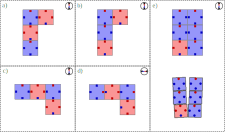
\includegraphics[width=0.80\textwidth]{figures/polyominoes.pdf}
	\caption{Polyominoes.}
	\label{fig:polyominoes}
\end{figure}

\section{Polyominoes}

%polyominoes. Fixed polys. Illegal polyominoes. Single cubes trivial polys, 


\begin{figure}
	\centering
	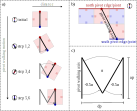
\includegraphics[width=0.80\textwidth]{figures/pivot_walking.pdf}
	\caption{This figure describes the pivot walking motion in detail. a) shows the six pivot walking steps for a single red cube. You can see the orientation of the magnetic field (bigger arrow indicates elevation). In b) an example polyomino with its pivot axis, edges and points is shown. c) illustrates the rotation of the pivot axis labeled with all the pivot walking parameters.}
	\label{fig:pivot_walking}
\end{figure}

\section{Motion}
In \cite{Bhattacharjee2022} three motion modes are presented. Rotation, pivot walking and rolling.
If the magnetic field orientation lays in the plane of the workspace, a rotation inside the plane forces all cubes to realign with the magnetic field.
Without any inclination of the magnetic field this rotation is performed around the center of mass for all polyominoes and we consider this motion a normal rotation.
Rotating the magnetic field perpendicular to the workspace plane, cubes can role forwards or backwards.
This rolling motion becomes problematic for self-assembly, because the top and bottom face of the cube, which contain no magnets, can become a side face.
Because rotation and pivot walking are sufficient enough to reach any position in the workspace, we don't consider rolling in our simulation and planning algorithms.
Elevating the magnetic field orientation by lifting up the south pole slightly, all polyominoes will pivot on the north face bottom edges of their most north placed cubes.
Pulling up the north pole does the opposite. The polyominoes will pivot on the south face bottom edges of their most south placed cubes.
The sum of all these cube edges are called the north or south pivot-edge and by keeping the magnetic field elevated and rotating around the normal vector of the workspace plane, the polyominoes will rotate around the center point of their pivot-edge.
This point is called the north or south pivot-point or foot.
All these edges and points are illustrated in figure \ref{fig:pivot_walking} b).

\begin{figure}
	\centering
	\includegraphics[width=0.80\textwidth]{figures/displacement_pivot_walking.png}
	\caption{All 19 four-cube polyomino shapes with their displacement vector $\vec{d}$ for one pivot walking cycle. $\vec{d}$ is drawn from the center of mass (red dot). North and south pivot foot are drawn as blue and brown dots.}
	\label{fig:displacement_pivot_walking}
\end{figure}

\paragraph{pivot walking:}
The principle of not rotating around the center of mass is important for pivot walking.
In the first step of a pivot waking cycle the magnetic field is elevated to let the polyomino pivot on its north pivot edge.
As a second step a rotation of $-\frac{1}{2} \cdot \alpha$ is performed around the north pivot point.
$-\pi \leq \alpha \leq \pi$ is the pivot walking angle.
For step 3 and 4 the elevation changes to its opposite to perform a rotation of $\alpha$ around the south pivot point.
Step 5 and 6 are equal to 1 and 2 and will bring the polyomino back to its original orientation.
You can see the pivot walking cycle steps in figure \ref{fig:pivot_walking} a) and have a closer look at its parameters in figure \ref{fig:pivot_walking} c).
In the end one pivot walking cycle moved the polyomino by a displacement vector $\vec{d}$ with $\lVert \vec{d} \rVert = d_p$, so $d_p$ is the distance the polyomino moved.
The direction and length of $\vec{d}$ changes with the shape of the polyomino.
The movement is always perpendicular to the pivot walking axis $\vec{a}$ with $\lVert \vec{a} \rVert = a_p$ , which is the vector between the north and the south pivot point, visualized in figure \ref{fig:pivot_walking} b).
$d_p$ can be calculated as following:
\begin{equation*}´
d_p = sin(\frac{1}{2} \cdot \alpha) \cdot a_p
\end{equation*}
To calculate $\vec{d}$ you can take the perpendicular of $\vec{a}$ and scale it to the length $d_p$.
To do a pivot walk left or right you can choose a negative or positive $\alpha$.
When you choose a big $\alpha$ according to amount, $d_p$ becomes also bigger, but the polyomino needs more space to the north and south to perform the rotations.
So for better maneuvering smaller values of $\alpha$ are preferable.
There is a strong deviation of length and direction of the displacement for different polyomino shapes.
So moving left or right might not move two polyominoes in the exact same direction.
In figure \ref{fig:displacement_pivot_walking} all 19 four-cube polyomino shapes with their displacement vectors are shown.

